%%%%%%%%%%%%%%%%%%%%%%%%%%%%%%%%%%%%%%%%%%%%%%%%%%%%%%%%%%%%%%%%%%%%%
%%%
%%% Set these variables appropriately
%%%
\newcommand{\AUTHORS}{Claudia V. Roberts}
\newcommand{\TITLE}{Detection of Weak Tor and Onion Keys in Tor Relay Servers}
\newcommand{\KEYWORDS}{Tor, RSA}
\newcommand{\CONFERENCE}{}
\newcommand{\PAGENUMBERS}{yes}       % "yes" or "no"
\newcommand{\TOAPPEAR}{no}
%%%
%%%
%%%%%%%%%%%%%%%%%%%%%%%%%%%%%%%%%%%%%%%%%%%%%%%%%%%%%%%%%%%%%%%%%%%%%

%%%% Setup the document/page
\documentclass[pdftex,twoside,twocolumn,11pt,letterpaper]{article}
\usepackage{ifthen}

\ifthenelse{\equal{\PAGENUMBERS}{yes}}{%
\usepackage[nohead,
            left=1in,right=1in,top=1in,
            footskip=0.5in,bottom=0.75in     % Room for page numbers
            ]{geometry}
}{%
\usepackage[noheadfoot,columnsep=0.2in,
            margin=1in,centering,truedimen]{geometry}
}

\usepackage{fancyhdr}
\usepackage[numbers,sort]{natbib}
\usepackage{xspace}
\usepackage{booktabs}
\usepackage{subfigure}
\usepackage[T1]{fontenc}
\usepackage{textcomp}
\usepackage{mathptmx}   % Times + Times-like math symbols
\usepackage{courier}
\usepackage[scaled=0.92]{helvet}

\usepackage{color}
\usepackage[pdftex]{graphicx}
\ifthenelse{\isundefined{\wantBW}}{%
  \usepackage[colorlinks]{hyperref}%        % for online version
}{%
  \usepackage[pdfborder={0 0 0}]{hyperref}% % for paper (B&W) version
}
\newcommand{\URL}[1]{\url{#1}}

%%%%% Setup for PDF
\hypersetup{%
pdfauthor = {\AUTHORS},
pdftitle = {\TITLE},
pdfsubject = {\CONFERENCE},
pdfkeywords = {\KEYWORDS},
bookmarksopen = {true}
}

%\setlength{\parindent}{0pt}
%\setlength{\parskip}{0pt}
\renewcommand{\headrulewidth}{0pt}
\newcommand{\Paragraph}[1]{\vspace{-2ex}\paragraph{#1.}}
\setlength{\topmargin}{-.15in}

\ifthenelse{\equal{\PAGENUMBERS}{yes}}{%
  \pagestyle{plain}
}{%
  \pagestyle{empty}
}

\makeatletter\long\def\@makecaption#1#2{
   \vskip 10pt
   \setbox\@tempboxa\hbox{\textsf{#1: #2}}
   \ifdim \wd\@tempboxa >\hsize % IF longer than one line:
       \textsf{#1: #2}\par      % THEN set as ordinary paragraph.
     \else                      % ELSE  center.
       \hbox to\hsize{\hfil\box\@tempboxa\hfil}
   \fi}
\makeatother

\clubpenalty=10000  % Don't allow orphans
\widowpenalty=10000 % Don't allow widows

\title{\textbf{\TITLE}}
\author{\AUTHORS}
\date{}

% Compact itemize and enumerate.  Note that they use the same counters and
% symbols as the usual itemize and enumerate environments.
\def\compactify{\itemsep=0pt \topsep=0pt \partopsep=0pt \parsep=0pt}
\let\latexusecounter=\usecounter
\newenvironment{CompactItemize}
  {\def\usecounter{\compactify\latexusecounter}
   \begin{itemize}}
  {\end{itemize}\let\usecounter=\latexusecounter}
\newenvironment{CompactEnumerate}
  {\def\usecounter{\compactify\latexusecounter}
   \begin{enumerate}}
  {\end{enumerate}\let\usecounter=\latexusecounter}

\newcommand{\comment}[1]{\textcolor{red}{#1}}
\newcommand{\ignore}[1]{}

\newcommand{\xc}[1]{\mbox{\textit{#1}}}
\newcommand{\la}{\leftarrow}
\newcommand{\ra}{\rightarrow}
\newcommand{\somespace}{\hspace{0.1cm}}

\def\discretionaryslash{\discretionary{/}{}{/}}
\def\discretionarydot{\discretionary{.}{}{.}}
\def\discretionarycolon{\discretionary{:}{}{:}}
{\catcode`\/\active
\catcode`\.\active
\catcode`\:\active
\gdef\URLprepare{\catcode`\/\active\let/\discretionaryslash
                 \catcode`\.\active\let.\discretionarydot
                 \catcode`\:\active\let:\discretionarycolon
        \def~{\char`\~}}}%
\def\URL{\bgroup\URLprepare\realURL}%
\def\realURL#1{\tt #1\egroup}%

\newcommand{\eg}{{\em e.g.}, }
\newcommand{\ie}{{\em i.e.}, }
\newcommand{\etal}{{\em et al.\ }}

\def\check{\stackrel{{\scriptscriptstyle ?}}{=}}

\begin{document}
\maketitle

\begin{abstract}
In its more than ten years of existence, the Tor network has seen hundreds of
thousands of relays come and go.  Each relay maintains several RSA keys,
amounting to millions of keys, all archived by The Tor Project.
%
In this paper, we analyze 3.7 million RSA public keys of Tor relays.  We \first
check if any relays share prime factors or moduli, \second identify relays that
use non-standard exponents, and \third characterize malicious relays that we
discovered in the first two steps.
%
Our experiments revealed that ten relays shared moduli, and 3,557
relays---almost all part of a research project---shared prime factors, allowing
adversaries to reconstruct private keys.  We further discovered 122 relays that
used non-standard RSA exponents, presumably in an attempt to attack onion
services.  By simulating how onion services are positioned in Tor's distributed
hash table, we identified four onion services that were likely targeted by these
malicious relays.
\end{abstract}
   
\section{Introduction}
\label{sec:intro}
Tor is a distributed overlay network designed to anonymize TCP-based applications such as web browsing, secure shell, and instant messaging~\cite{dingledine2004tor}. Its goal is to protect the privacy of its users and defend them against traffic analysis, a form of network surveillance. In order to provide this anonymity, data packets are sent through a multi-hop virtual circuit of nodes called relays or onion routers. By using a separate set of encryption keys for each hop, these encrypted relay circuits ensure that no observer at a single point along the communication channel can directly identify both the true source and the final destination. While many users are using Tor for its intended purpose--to prevent Internet Service Providers (ISPs) from learning their online browsing habits, to aid law enforcement in sting operations, and to allow human rights activists to anonymously report abuses from danger zones~\cite{torusers}--it is no surprise that there are others using it to facilitate their illegal activities. This has made Tor a target for deanonymization attacks by governmental adversaries, such as the NSA and FBI, and ISPs whose aim is to deanonymize Tor users and link them back to their online activity. The Tor project openly welcomes academic research that helps defend it from such attacks as well as research that helps expose unknown vulnerabilities in its anonymous communication system.

Tor relies on the Transport Layer Security (TLS) protocol and asymmetric key cryptography to encrypt messages that travel between the nodes of the Tor relay circuits. In RSA public-key cryptography, the strength of the system depends on the degree of difficulty for which a generated private key can be determined from its corresponding public key. Factors such as the length of the key and the strength of the random number generator during key generation have proven to be critical to the security of modern cryptographic systems~\cite{rivest1978method, heninger2012mining, lenstra2012ron}. In 2012,~\cite{heninger2012mining, lenstra2012ron} conducted what were at the time the largest network surveys of TLS and SSH servers.~\cite{heninger2012mining} found an alarmingly large number of vulnerable RSA public keys and claimed to have computed the RSA private keys for 0.50\% of TLS hosts. The research group pinpointed the underlying issue to malfunctioning random number generators. More specifically,~\cite{heninger2012mining} traced the vulnerable keys to resource-constrained network devices which had not been properly seeded with adequate amounts of entropy. From their analysis of over 12 million TLS hosts and over 10 million SSH hosts,~\cite{heninger2012mining} identified three types of vulnerabilities: repeated keys, factorable RSA keys, and repeated ephemeral keys in DSA signatures. In all three cases, the problems were tied to specific faulty key generation implementations caused by insufficient entropy.

Tor has grown to become the most popular and well-researched anonymity network consisting of over 2 million directly connecting users and over 7,000 volunteer-operated Tor relay severs~\cite{metrics}. While many of the relays run on large PCs and VPS data centers, there is anecdotal evidence that some relays run on smaller devices such as Raspberry Pi products. This poses a potential risk to the anonymity of Tor because resource-constrained machines are more susceptible to generating weak RSA public keys~\cite{heninger2012mining, lenstra2012ron}. In order to detect potentially weak factorable keys in Tor, I used~\cite{heninger2012mining}'s fastgcd solution for efficiently computing the greatest common divisor for every pair of integers in a large set. While it is not computationally practical to factor large integer RSA keys, it is computationally practical to compute their pair-wise GCDs. Thus, if an attacker is able to find a pair of RSA key moduli with shared prime factors, then she can easily use this information to compute the private keys~\cite{heninger2012mining, lenstra2012ron}. Knowing the private key of a Tor relay server has serious security implications, and is a critical first step to compromising the anonymity of the system. With private key in hand, that adversary now has control of the relay.

In Section 2 I provide background. In Section 3 I discuss my methodology. In Section 4 I provide evaluation. In Section 5 I discuss future work, and in Section 6 I conclude.
\section{Background}
We now provide brief background on both the RSA cryptosystem and how the Tor
network employs RSA.

\subsection{The RSA cryptosystem}
The RSA public key cryptosystems is comprised of two keys: a public encryption
key and a privately held decryption key. The encryption key---or RSA public
key---is comprised of a pair of positive integers, an exponent $e$ and a modulus
$N$. The modulus $N$ is the product of two large, random prime numbers $p$ and
$q$. The corresponding decryption key---or RSA private key---is comprised of the
positive integer pair $d$ and $N$ where $d = e^{-1}$ mod $(p - 1)(q - 1)$.  The
decryption exponent $d$ is efficient to compute if the factorization of $N$ is
known.

The security of RSA rests upon the difficulty of factorizing $N$ into its prime
factors $p$ and $q$.  While factoring $N$ is impractical given sufficiently
large prime factors, the greatest common divisor (GCD) of \emph{two moduli} can
be computed in mere microseconds.  Consider two distinct RSA moduli $N_1 = pq_1$
and $N_2 = pq_2$ that share the prime factor $p$.  An attacker could quickly and
easily compute the GCD of $N_1$ and $N_2$ in order to obtain $p$, then divide
the moduli by $p$ to determine $q_1$ and $q_2$, thus compromising the private
key of both key pairs.  Therefore, it is crucial that both $p$ and $q$ are
determined using a strong random number generator.

\subsection{The Tor network}
As of January 2017, the Tor network consists of almost 7,000
relays~\cite{tormetrics}.  Each of these relays maintains RSA, Curve25519, and
Ed25519 key pairs~\cite[\S~1.1]{torspec}.  We are only interested in the
RSA key pairs, whereof relays have the following three.  All three key pairs use
1024-bit keys.

\begin{description}
    \item[Identity key]  Relays have a long-term identity key that they only use
        to sign documents and certificates.  Relays are frequently referred to
        by their fingerprint, which is a hash over their identity key.  The
        compromise of an identity would allow an attacker to entirely
        impersonate a relay, \eg, by publishing spoofed descriptors.
    \item[Onion key]  Relays use medium-term onion keys to decrypt cells when
        circuits are created.  The RSA-based onion key is only used in the Tor
        Authentication Protocol that is now superseded by the ntor handshake.  A
        compromised onion key allows the attacker to read the content of cells
        until the key pair rotates.
    \item[Connection key] The short-term connection keys protect the connection
        between relays using TLS.  Connection keys are rotated at least once a
        day.  The TLS connection provides defense in depth.  If compromised, an
        attacker is able to read the cells that are exchanged between Tor
        relays.
\end{description}

In our work, we only consider the three 1024-bit RSA key pairs that each relay
has.  The Tor Project is archiving these key pairs since more than ten years,
allowing us to draw on a rich data set~\cite{collector}.

\section{Methodology}
\label{sec:methodology}

\subsection{Data collection}
Tor has many years' worth of RSA public keys from thousands of Tor relays. The first step I took was to use CollecTor, the Tor network data-collecting service, to collect all recent and archived relay server descriptors. Descriptors that were published in the last 72 hours are available as plain text, and archived descriptors covering over 10 years of Tor network history are available as compressed tarballs. Relay server descriptors contain information that relays publish about themselves such as their nickname, fingerprint, IPv4 address, operating system, Tor version, contact information, and most importantly, their signing key and onion key~\cite{collector}. The signing key is the relay's long-term RSA public identity key and the onion-key, also an RSA public key, is used for short-term encryption. I used the Tor Stem Python controller library to collect all 3,763,821 RSA public keys (signing and onion) from the CollecTor repository of recent and archived server descriptors. It took less than 24 hours to unpack an estimated 200 GB worth of compressed archived relay server descriptor tarballs on a Princeton University computer science departmental machine. The machines used in this paper are all Fujitsu RX200 S8 servers with dual, eight-core 2.8GHz Intel Xeon E5 2680 v2 processors with 256GB RAM running the Springdale distribution of Linux~\cite{cscycles}.

During the key collection process, I serialized a Python dictionary that maps Tor RSA public keys to their relay descriptor metadata. I kept track of each key's relay nickname, identity key fingerprint, time when the descriptor was made, IPv4 address, onion routing port, operating system, tor version, contact information, average bandwidth, and hex encoded digest of extra information. I used this dictionary during my post-fastgcd weak key analysis (see Figure~\ref{rsa-relay}.

\begin{figure}[h]
\centering
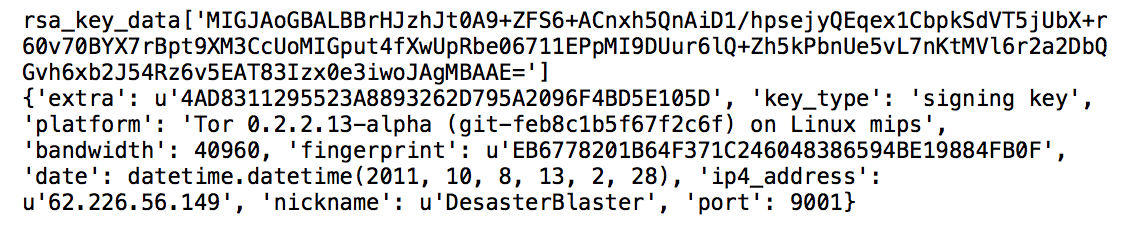
\includegraphics[width=\linewidth]{rsa-relay.png}
\caption{Tor RSA key metadata}
\label{rsa-relay}
\end{figure}

\subsection{Run fastgcd}
To detect potentially weak factorable keys in Tor, I used~\cite{heninger2012mining}'s fastgcd solution for efficiently computing the pair-wise GCD of 3,763,821 Tor public keys generated between December 2005 and December 2016. Fastgcd is a C implementation of an efficient quasilinear-time algorithm for factoring a collection of integers into co-primes. The algorithm is based on Bernstein's algorithm~\cite{bernstein2004find}. As input, fastgcd takes in a file containing a list of RSA moduli in hex. The algorithm computes the GCD of each input integer with the product of every other input integer and outputs two files. One file contains the list of input moduli that had a nontrivial common divisor with any input modulus, and the other file contains the list of common divisors of each vulnerable modulus. 

Before running the set of 3,763,821 RSA public keys through fastgcd, I had to run a few pre-processing steps. To properly extract the moduli from the public keys and convert them to hex, I had to find the lengths and encodings used for the signing and onion keys. After some investigation, I deduced that the Tor RSA keys are 1024-bit, PKCS\#1-padded, OpenSSL PEM-encoded keys~\cite{torspecbug}. The keys returned by Stem are pure RsaPublicKey objects comprised of a base64 ASN.1 sequence with two integers: a modulus N and exponent e. With this knowledge, I was able to use the PyCrypto Python package to properly extract the moduli and exponents from all Tor RSA public key as well as convert the moduli to hex. I ran fastgcd on this pre-processed list of 3,763,821 unique moduli. The program took less than 48 hours to run on Princeton's supercomputers.
\section{Evaluation}
\label{sec:eval}

In a survey of all 3,763,821 Tor relay server RSA public keys, I found that 0.60\% of all long-term signing keys had moduli with shared prime factors and found 10 long-term signing keys with repeated moduli. In an analysis of these weak keys, I was able to connect the 10 keys with repeated moduli to a 2014 attack against one of Tor's distributed hash tables and connected more than a third of the factorable RSA keys to a Tor hidden services research project conducted in 2013.

\subsection{Signing keys with shared prime factors}
Of the 588,947 long-term Tor relay identity keys, 0.60\% (3,577) were found to have moduli with shared prime factors. Of these 3,577, 37.13\% (1,321) were found to be directly connected to a 2013 hidden services research project where the authors created large number of Tor relays hosted on Amazon EC2 machines~\cite{biryukov2013trawling, sybil}.

This leaves 2,236 weak Tor signing keys with shared prime factors that are not directly connected to the 2014 hidden services research project. In order to gather more information on the relays, I ran the remaining 2,236 factorable keys through WHOIS. I present my findings below and visualize them in the following figures (see Figures~\ref{country-code-distro},~\ref{dist-across-os}, and~\ref{dist-3-yrs} ).

\begin{figure}[h]
\centering
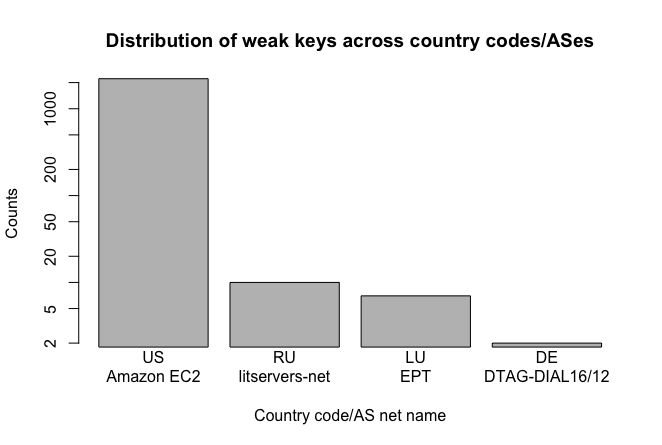
\includegraphics[width=\linewidth]{country-code-distribution.png}
\caption{Distribution of weak keys across country codes/ASes}
\label{country-code-distro}
\end{figure}


\begin{figure}[h]
\centering
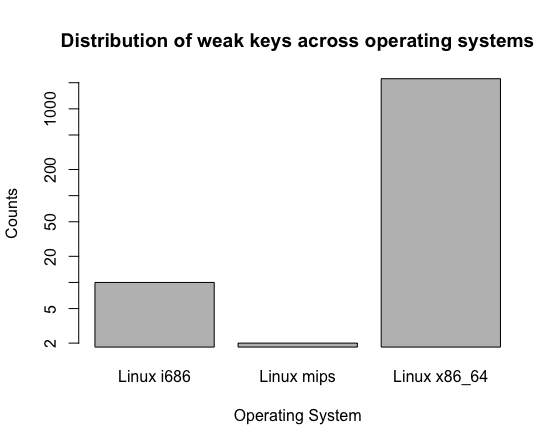
\includegraphics[width=\linewidth]{distribution-across-OS.png}
\caption{Distribution of weak keys across operating systems}
\label{dist-across-os}
\end{figure}


\begin{figure}[h]
\centering
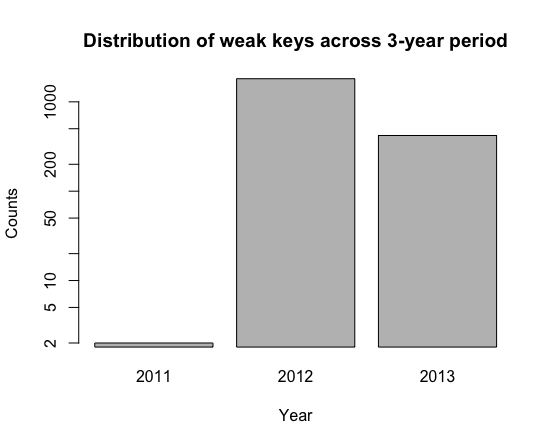
\includegraphics[width=\linewidth]{distribution-over-3-years.png}
\caption{Distribution of weak keys across 3-year period}
\label{dist-3-yrs}
\end{figure}

\begin{itemize}
    \item 2,217 of these 2,236 keys originated from Tor relay IP addresses with the US (United States) country code. Additionally, all of these originated from IP addresses with AMAZON-EC2 and AMAZON-ZIAD1 ASN net names.
    \item 10 of these 2,236 keys originated from Tor relay IP addresses with the RU (Russia) country code. Additionally, all of these originated from IP addresses with the litservers-net ASN net name. These Tor relays were published in November 2012.
    \item 7 of these 2,236 keys originated from Tor relay IP addresses with the LU (Luxembourg) country code. Additionally, all of these originated from IP addresses with the EPT ASN net name. These Tor relays were generated in November 2012. The authors~\cite{biryukov2013trawling} conducted their research at the University of Luxembourg.
    \item 2 of these 2,236 keys originated from Tor relay IP addresses with the DE (Germany) country code. Additionally, all of these originated from IP addresses with DTAG-DIAL16 and DTAG-DIAL12 ASN net names. These Tor relays were generated in late 2011.
\end{itemize}


\subsection{Signing keys with repeated moduli}
To my surprise, during my experiment, I found 10 Tor signing keys with repeated moduli. Their RSA public keys were distinct but their moduli were identical. I traced these keys to a 2014 attack against Tor's distributed hash table that's used for onion services.
\section{Future Work}
\label{sec:future}

I plan to continue investigating this research problem along with my advisers. I have reached out to the authors of~\cite{biryukov2013trawling} to ask if they were aware that they were generating RSA public keys with shared prime factors, and if so, what was their reasoning behind this. I also asked them if they hosted the Tor relays on any other machines besides Amazon EC2. One of the authors has replied and has agreed to look into the issue. Given that I detected over 3,000 factorable keys, the next step is to attempt to compute some of the private keys. Finally,~\cite{heninger2012mining} cite that the fastgcd algorithm is able to factor more keys if you serve it a larger collection of inputs since it will have a larger factor base to use on each key.~\cite{hastings2016weak} successfully extracted 81 million distinct RSA keys. I will re-run fastgcd using all Tor signing and onion keys in conjunction with these 81 million distinct RSA keys to detect whether there are more vulnerable Tor keys than I originally found in this paper.
\section{Conclusions}
\label{sec:conclusion}

In order to detect potentially weak factorable keys in Tor, I used~\cite{heninger2012mining}'s fastgcd solution for efficiently computing the greatest common divisor for every pair of integers in a large set. While it is not computationally practical to factor large integer RSA keys, it is computationally practical to compute their pair-wise GCDs. Thus, if an attacker is able to find a pair of RSA key moduli with shared prime factors, then she can easily use this information to compute the private keys~\cite{heninger2012mining, lenstra2012ron}. Knowing the private key of a Tor relay server has serious security implications, and is a critical first step to compromising the anonymity of the system. With private key in hand, that adversary now has control of the relay. In a survey of all 3,763,821 Tor relay server RSA public keys, I found that 0.60\% of all long-term signing keys had moduli with shared prime factors and found 10 long-term signing keys with repeated moduli. I will continue my quest to protect the anonymity of Tor users by extending my work on this project.
\section*{Acknowledgments}
A big thank you to my advisers Philipp Winter, Laura M. Roberts, and Yorgos Kadianakis.

%% Bibliography
%\vspace{-1ex}
%\linespread{1.0}
%\setlength{\bibsep}{1pt}
%\footnotesize
\small
\bibliography{local}
\bibliographystyle{abbrvnat}

\end{document}

